\section{Résultats}

\begin{figure}
    \centering
    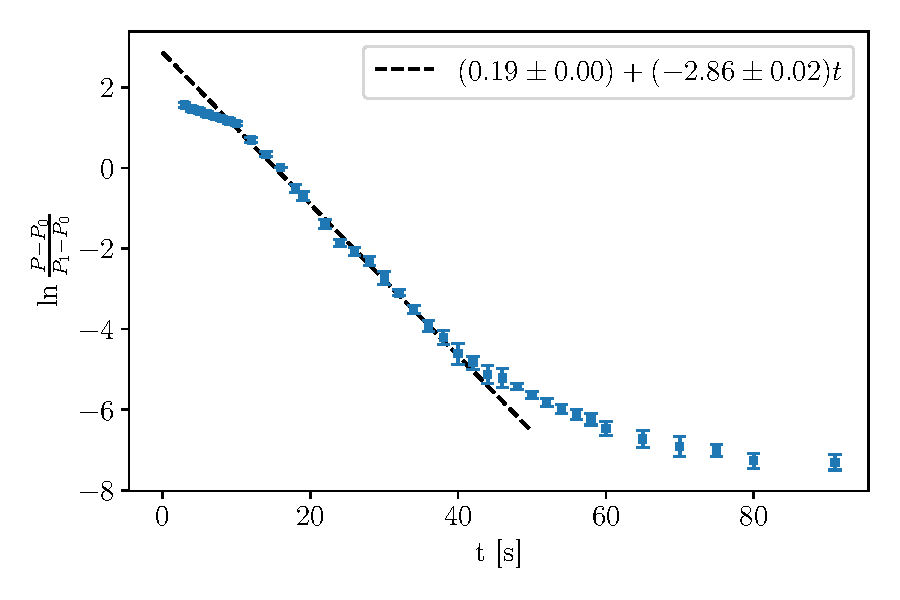
\includegraphics[width=0.5\linewidth]{figures/cinetique_palettes.pdf}
    \caption{Suce ma pompe}
    \label{fig:cinetique_palette}
\end{figure}

\paragraph*{Cinétique pompe à palettes}
La pression dans la chambre de volume \(V = (5.5 \pm 0.5)\) \si{\milli\bar} en fonction du temps est donné dans la \autoref{fig:cinetique_palette}. Une régression linéaire sur les points 12 à 40 permet d'obtenir une valeur moyenne sur \(\ln{\frac{P - P_0}{P_1 - P_0}}\) avec laquelle il est possible d'obtenir avec l'\autoref{eq:cinetique} le débit effectif \(S = (1.12 \pm 0.01)\) \si{\liter \per \second}.

\paragraph*{Cinétique pompe à diffusion}

 





 \\



\begin{figure}
    \centering
    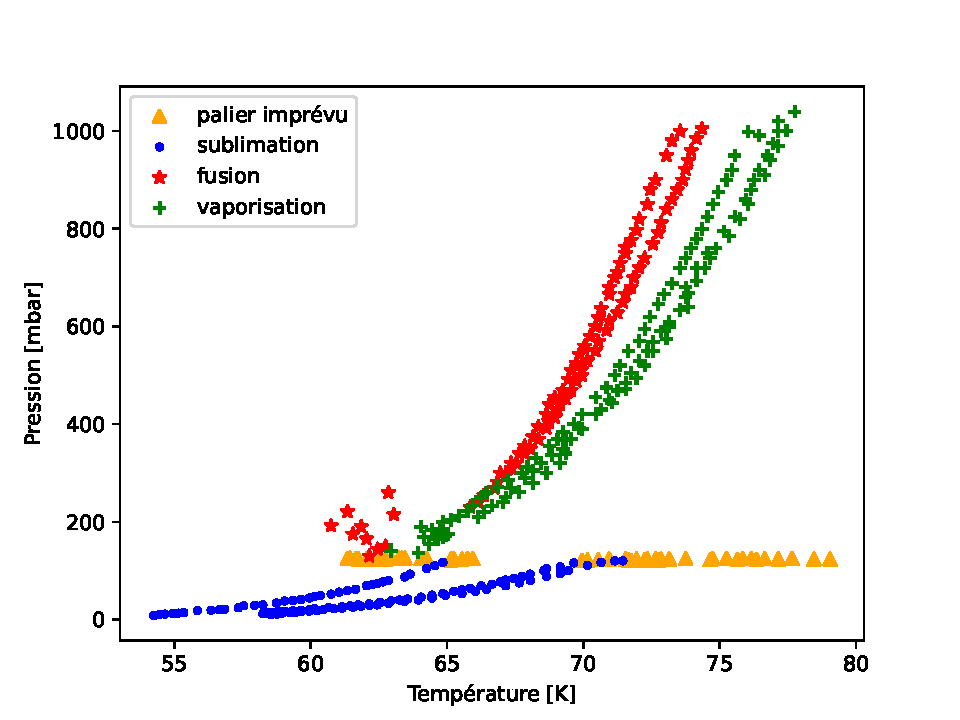
\includegraphics[width=0.6\textwidth, height=7cm]{figures/etats_azote_all_data.pdf}
    \caption{Points de cohabitation de deux états de l'azote}
    \label{fig:alldata}
\end{figure}

Pour la deuxième partie de l'expérience l'étude des changements d'état de l'azote à volume constant a été effectuée. Cinq ensembles de mesure ont été pris successivement en arrêtant le pompage à différents moments. Il est important de noter que l'installation disponible au moment de l'exécution de l'expérience manquait d'un agitateur utile pour homogénéiser le mélange. A plusieurs moments durant les mesures il a donc été possible d'observer une cohabitation des trois états même en dehors du point triple, les conditions de température n'étant pas les même dans tout le volume. \\
Une première mesure de la courbe de sublimation avec arrêt du pompage après solidification complète et refroidissement en dessous de 55 \si{\kelvin} a été effectuée. Celle-ci s'est poursuivie par une mesure de la courbe de fusion sans disparition complète de l'azote solide. Les deux autres mesures de la courbe de sublimation se sont poursuivies par un palier inattendu entre 121 et 126 \si{\milli \bar}. La fin de ce palier a été caractérisé à deux reprises par un saut important dans les données (\(\Delta T = 15\) \si{\kelvin} en 12 \si{\second}) et a été suivi par le relevé d'une courbe de vaporisation. Deux autres mesures ont été effectuées, l'une après la solidification complète de l'azote liquide afin de relever une courbe de fusion supplémentaire et l'autre juste au début de la solidification afin de relever une autre courbe de vaporisation. L'ensemble des mesures est présenté dans la \autoref{fig:alldata}. \\
\\
Afin d'obtenir des courbes de changement d'état plus claires les données obtenues ont été sélectionnées. La courbe de sublimation non-polluée par un palier a été gardée. Le palier a été entièrement retiré et les points des courbes de fusion à des températures inférieures au point triple (65 \si{\kelvin}), qui correspondent à des variations du système au point triple, ont également été supprimés. Ce traitement des données a permis d'obtenir la \autoref{fig:cleandata}.

POINT TRIPLE TMIN


\begin{figure}
    \centering
    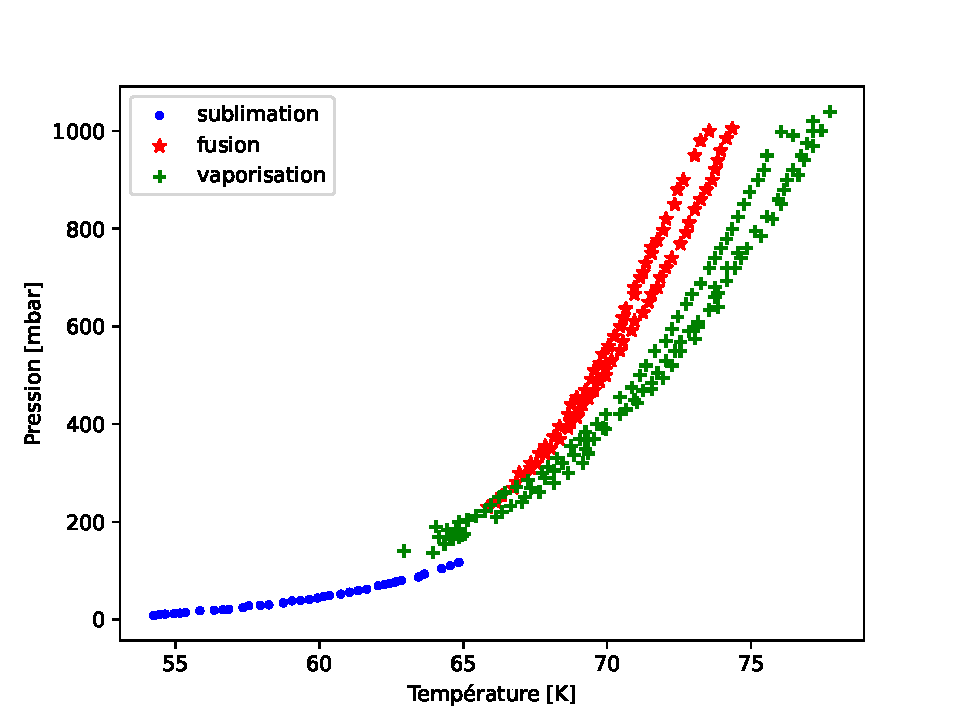
\includegraphics[width=0.6\textwidth, height=7cm]{figures/etats_azote_clean.pdf}
    \caption{Courbes de changement d'état de l'azote}
    \label{fig:cleandata}
\end{figure}




